%=====================================================================================================
%=====================================================================================================
\chapter{Complexity Analysis of the UAV Path Planning Problem}
\label{chap:complexity}

In this appendix, we analyze why a heuristic approach is preferred to a dynamic programming / reinforcement learning approach by comparing the computational complexity of each approach.

%=====================================================================================================
\section{Computational Complexity of Dynamic Programming}
\label{DPComplexity}

The key issue is that the path planning problem that we are solving cannot be solved in polynomial time using dynamic programming unless P=NP\footnote{The path planning problem we are solving is similar to the Orienteering Problem (OP), which can be seen as a combination between the Knapsack Problem (KP) and the Traveling Salesman Problem (TSP). In a fully connected graph where each vertex has a certain score (prize), with fixed starting vertex and end vertex, the OP problem asks for the path that would achieve the highest score within a given time frame. That is why the OP problem is also called the Prize-Collecting TSP problem and TSP with profits. Scores are entirely additive and each vertex can only be visited once (not all vertices have to be visited). OP, like TSP, is an NP-hard problem.

Our path planning problem is different from the OP problem in the following aspects: (a) we use a grid representation because this is compatible with UAV flight, so the search is on a graph that is not a complete graph (fully connected); (b) the Bayesian sensing of the UAVs sensors require that the path planning be able to visit the same vertex repeatedly; and (c) this means that the ``prize'' rewarded for each visit to a vertex is only partially collected and is path dependent.}. The justification for this is as follows:

\begin{itemize}
\item The problem that we are solving is at least as computationally complex as what is known as the Orienteering Problem.  
\item The Orienteering Problem is at least as computationally complex as the Traveling Salesperson Problem.
\item The Traveling Salesperson Problem is in the complexity class f-NP, with its corresponding decision problem in the class NP-complete.
\item By reduction, this means that our path planning problem is NP-hard and cannot be solved in polynomial time unless P=NP.
\item Because the path-planning problem is NP-hard, we cannot solve it using dynamic programming in real time for the planning lengths that we consider (up to 900 planning steps).
\end{itemize}

%=====================================================================================================
\section{Complexity of Reinforcement Learning (Approximate Dynamic Programming)}
\label{RLComplexity}

Reinforcement learning cannot learn an optimal solution to an NP-hard problem in polynomial time\footnote{The approximate dynamic programming / reinforcement learning (ADP/RL) approach does not support (near) real-time solution. For example, Righini and Salanil show in~\cite{Righini2009Decremental} that it takes roughly 1000-3000 seconds to solve an OP type problem with 100 vertices/nodes. The ADP/RL approach also does not scale well due to its complexity. Vansteenwegen et al.\ surveyed different approaches to solving the OP~\cite{Vansteenwegen2011Orienteering}. Most of the approaches were heuristic approaches, and the only ADP/RL approach mentioned is~\cite{Righini2009Decremental}.}. If it could, then P=NP. Moreover, reinforcement learning typically requires many, many iterations to reach convergence even for moderately sized problems, meaning it is likely to be significantly slower.  Even dynamic programming-based approaches to reinforcement learning, like learning the transition model and applying policy iteration, cannot run in polynomial time on an exponential problem.

In addition to this fundamental limitation of what reinforcement learning can theoretically do, there is a second practical problem with using reinforcement learning for this problem. This practical limitation is that reinforcement learning approaches tend to get stuck in local minima when there are multiple rewards in the problem.  Indeed, the literature includes many papers that seek to resolve this problem by trading off exploration and exploitation~\cite{Sutton1998Reinforcement}.  These approaches work in practice for some problems, but there is no evidence that these approaches will work for problems that are exponentially complex.  

Moreover, the state space of our path-planning problem grows exponentially because of the possibility of revisiting states. For each revisit, a new reward function must be defined because the Bayesian approach allows for partial collection of information.  This means that we end up with an exponentially hard problem with an exponentially large state space and a unique reward for each element of the state space.  There is no known reinforcement learning algorithm that can solve such problems, let alone solve it in real-time.

%=====================================================================================================
\section{Classical Dynamic Programming for Our UAV Path Planning Problem}
\label{CDPUAV}

Classical dynamic programming (DP) is a method for solving complex problems by breaking them down into simpler subproblems. Solution to subproblems can be stored to trade space for time. Problems that can be solved by DP must exhibit two key attributes: optimal substructure and overlapping subproblems. For example, the DP method can be used to find the exact solution for the TSP problem with few nodes. However, since the TSP problem is NP-hard, it cannot be solved in polynomial time, unless P=NP. Therefore, even with the DP method, the complexity is still $O(2^n n^2)$~\cite{Bellman1958Combinatorial}. DP method suffers the ``curses of dimensionality'' and does not scale well with complex problems.

Our path planning problem can be reduced to the OP; therefore, the problem is also at least NP-hard. Our path planning problem has a state space of 10,000 nodes and a flight path of 900 (possibly higher in real application) time steps, meaning that theoretically the same node could be visited 900 times. If we treat each visit to the same node as a separate node, the state space expands to 9,000,000 nodes, and tracking the connectivity of all these nodes (not complete) also becomes intractable.

In order to support real WiSAR operations, we need to have the path created within seconds. Also in practical Wilderness Search and Rescue scenarios, the search area could be much bigger than the 10,000 nodes we demonstrated. The UAV flight time can also be much longer depending on the type of UAV platforms used. That's why we chose a heuristic approximation approach in solving this problem. The complexity of our approach is $O(n)$ once we have the Mode Goodness Ratio (MGR) heuristic, where $n$ is the flight duration in time steps ($n$=900 in our scenarios). This means our approach is very fast and scales very nicely with the NP-hard problem.


%=====================================================================================================
\section{Reinforcement Learning (Approximate Dynamic Programming) for Our UAV Path Planning Problem}
\label{RLUAV}

Instead of solving for the exact solution, approximate dynamic programming / reinforcement learning (ADP/RL) are approximate methods to search for solutions that approximate the optimal solution for complex problems to avoid the ``curses of dimensionality''. ADP/RL methods have four main sub-elements: a policy, a reward function (immediate payoff), a value function (long-term payoff), and optionally, a model of the environment. A policy defines the learning agent's behavior at a given time, a reward function defines the goal and indicates what is good in an immediate sense, a value function specifies what is good in the long run, and, the model of the environment mimics the behavior of the environment. The idea is to learn the optimal policy iteratively for each state, balancing exploration and exploitation. ADP/RL methods use Markov Decision Process (MDP) and can work with problems that have uncertainty in transition.

In our path planning problem, a node can be visited multiple times, and because our Bayesian approach allows for partial collection of information, the score/prize collected for each visit is different. The reward function and the value function both become path dependent, the state space becomes exponentially large. As described in the previous section, we need real time solutions that scale well when search area and flight duration expand.

%=====================================================================================================
%=====================================================================================================
\chapter{Full Experiment Results for Chapter 5}
\label{chap:result}

Here we present the full experiment results of the four WiSAR scenarios described in Chapter 5. For each scenario, we generate paths with three flight durations ($T=300$, $T=600$, and $T=900$) and compare algorithm computation speed (in seconds) and path $\mathit{Efficiency_{LB}}$ (in \%) for BA, LHC-GW-CONV, Top2, and TopN algorithms (including Top2 and TopN algorithms where $k=5$ and $N=3$). All numbers shown are averages of 10 runs. Best performance results are displayed in bold font face. Standard deviations ($\sigma$) are also shown for both computation speed and path $\mathit{Efficiency_{LB}}$.

%=============
% TestCase
%=============

Table~\ref{TestCaseTable} shows the experiment results for the synthetic WiSAR scenario with a multi-modal distribution of the missing person location and a simple task-difficulty map with three difficulty levels (as shown in Fig.~\ref{SyntheticCase}). The UAV path starts from a subregion with high task-difficulty (lower right corner).

\begin{center}
\begin{table*}[hbtp]
{
%\small
\scriptsize
\hfill{}
\setlength{\extrarowheight}{1.5pt}
\begin{tabular}
{|l|c|c|c|c|c|c|c|c|c|c|c|c|}
\hline
& \multicolumn{4}{|c|}{$T=300$} & \multicolumn{4}{|c|}{$T=600$} & \multicolumn{4}{|c|}{$T=900$} \\ 
\hline
& Speed & $\sigma$ & $\mathit{E_{LB}}$ & $\sigma$ & Speed & $\sigma$ & $\mathit{E_{LB}}$ & $\sigma$ & Speed & $\sigma$ & $\mathit{E_{LB}}$ & $\sigma$\\ 
\hline
BA & - & - & 27.59 & - & - & - & 43.54 & - & - & - & 59.56 & - \\ 
\hline
LHC-GW-CONV & 0.17 & 0.01 & 92.26 & 0.00 & 0.33 & 0.07 & 92.68 & 0.00 & 0.51 & 0.09 & 94.03 & 0.01 \\ 
\hline
Top2 (1 layer) & 0.12 & 0.05 & 87.49 & 0.03 & 0.14 & 0.04 & 91.66 & 0.04 & 0.15 & 0.04 & 91.02 & 0.03 \\ 
\hline
TopN (1 layer) & \textbf{0.10} & 0.05 & 91.28 & 0.02 & \textbf{0.08} & 0.05 & 91.93 & 0.04 & \textbf{0.07} & 0.03 & 95.24 & 0.01 \\ 
\hline
Top2 (Hierarchy) & 0.37 & 0.10 & 90.85 & 0.02 & 0.42 & 0.10 & 93.83 & 0.02 & 0.48 & 0.10 & 93.59 & 0.01  \\ 
\hline
TopN (Hierarchy) & 0.91 & 0.21 & \textbf{92.27} & 0.00 & 0.84 & 0.16 & \textbf{95.50} & 0.01 & 0.93 & 0.21 & \textbf{95.56} & 0.01 \\ 
\hline
\end{tabular}}
\medskip
\caption{Algorithms speed and $\mathit{Efficiency_{LB}}$ comparison for the multi-modal synthetic scenario.}
\label{TestCaseTable}
\vspace*{-5ex}
\end{table*}
\end{center}

%=============
% HikerPaul
%=============

Table~\ref{HikerPaulTable} shows the experiment results for the HikerPaul WiSAR scenario, in which an elderly couple was reported missing near the Grayson Highlands State Park in Virginia. Fig.\ref{HikerPaulMaps} shows the probability distribution map and the task-difficulty map for the scenario. Fig.\ref{HikerPaulPaths} shows example paths generated. Each UAV path starts from the Last Known Position (LKP), which is in the middle of the search region.

\begin{center}
\begin{table*}[hbtp]
{
%\small
\scriptsize
\hfill{}
\setlength{\extrarowheight}{1.5pt}
\begin{tabular}
{|l|c|c|c|c|c|c|c|c|c|c|c|c|}
\hline
& \multicolumn{4}{|c|}{$T=300$} & \multicolumn{4}{|c|}{$T=600$} & \multicolumn{4}{|c|}{$T=900$} \\ 
\hline
& Speed & $\sigma$ & $\mathit{E_{LB}}$ & $\sigma$ & Speed & $\sigma$ & $\mathit{E_{LB}}$ & $\sigma$ & Speed & $\sigma$ & $\mathit{E_{LB}}$ & $\sigma$\\ 
\hline
BA & - & - & 56.95 & - & - & - & 60.07 & - & - & - & 57.11 & - \\ 
\hline
LHC-GW-CONV & 0.30 & 0.16 & 60.18 & 0.13 & 0.47 & 0.03 & 56.76 & 0.00 & 0.98 & 0.16 & 55.18 & 0.00\\ 
\hline
Top2 (1 layer) & \textbf{0.24} & 0.06 & 66.68 & 0.09 & 0.30 & 0.11 & 65.21 & 0.07 & 0.41 & 0.20 & 66.08 & 0.07\\ 
\hline
TopN (1 layer) & 0.25 & 0.07 & 76.19 & 0.08 & \textbf{0.24} & 0.11 & 71.02 & 0.04 & \textbf{0.22} & 0.09 & 68.26 & 0.04\\ 
\hline
Top2 (Hierarchy) & 0.73 & 0.11 & 78.67 & 0.03 & 0.84 & 0.14 & 73.81 & 0.04 & 1.19 & 0.36 & 72.75 & 0.02\\ 
\hline
TopN (Hierarchy) & 1.52 & 0.15 & \textbf{81.43} & 0.03 & 1.73 & 0.25 & \textbf{75.48} & 0.02 & 1.68 & 0.26 & \textbf{74.13} & 0.02\\ 
\hline
\end{tabular}}
\medskip
\caption{Algorithms speed and $\mathit{Efficiency_{LB}}$ comparison for the HikerPaul scenario.}
\label{HikerPaulTable}
\vspace*{-2ex}
\end{table*}
\end{center}

%=============
% NewYork53
%=============

Table~\ref{NewYork53Table} shows the experiment results for the NewYork53 WiSAR scenario, in which a 46 year old male camper was reported missing near Adirondack Park in upperstate New York. Fig.\ref{NewYork53Maps} shows the probability distribution map and the task-difficulty map for the scenario. Fig.\ref{NewYork53Paths} shows example paths generated. Each path starts from the Last Known Position (LKP), which is in the middle of the search region.

\begin{center}
\begin{table*}[hbtp]
{
%\small
\scriptsize
\hfill{}
\setlength{\extrarowheight}{1.5pt}
\begin{tabular}
{|l|c|c|c|c|c|c|c|c|c|c|c|c|}
\hline
& \multicolumn{4}{|c|}{$T=300$} & \multicolumn{4}{|c|}{$T=600$} & \multicolumn{4}{|c|}{$T=900$} \\ 
\hline
& Speed & $\sigma$ & $\mathit{E_{LB}}$ & $\sigma$ & Speed & $\sigma$ & $\mathit{E_{LB}}$ & $\sigma$ & Speed & $\sigma$ & $\mathit{E_{LB}}$ & $\sigma$\\ 
\hline
BA & - & - & 39.95 & - & - & - & 54.27 & - & - & - & 65.08 & - \\ 
\hline
LHC-GW-CONV & \textbf{0.01} & 0.00 & 38.47 & 0.00 & \textbf{0.02} & 0.00 & 56.91 & 0.00 & \textbf{0.02} & 0.00 & 67.38 & 0.00\\ 
\hline
Top2 (1 layer) & 0.75 & 0.15 & 54.42 & 0.04 & 0.92 & 0.60 & 66.61 & 0.03 & 0.81 & 0.55 & 72.79 & 0.02\\ 
\hline
TopN (1 layer) & 0.70 & 0.45 & 59.15 & 0.07 & 0.77 & 0.55 & 68.78 & 0.04 & 0.69 & 0.30 & 74.54 & 0.01\\ 
\hline
Top2 (Hierarchy) & 1.87 & 0.23 & 57.18 & 0.03 & 2.06 & 0.34 & 69.29 & 0.02 & 1.92 & 0.33 & 74.44 & 0.01\\ 
\hline
TopN (Hierarchy) & 5.01 & 0.67 & \textbf{65.39} & 0.03 & 5.76 & 0.96 & \textbf{71.47} & 0.02 & 5.32 & 1.12 & \textbf{77.36} & 0.02\\ 
\hline
\end{tabular}}
\medskip
\caption{Algorithms speed and $\mathit{Efficiency_{LB}}$ comparison for the NewYork53 scenario.}
\label{NewYork53Table}
\vspace*{-5ex}
\end{table*}
\end{center}

%=============
% NewYork108
%=============

Table~\ref{NewYork108Table} shows the experiment results for the NewYork53 WiSAR scenario, in which two teenage female hikers were reported missing near West Chesterfield in Massachusetts. Fig.\ref{NewYork108Maps} shows the probability distribution map and the task-difficulty map for the scenario. Fig.\ref{NewYork108Paths} shows example paths generated. Each path starts from the Last Known Position (LKP), which is in the middle of the search region.

\begin{center}
\begin{table*}[hbtp]
{
%\small
\scriptsize
\hfill{}
\setlength{\extrarowheight}{1.5pt}
\begin{tabular}
{|l|c|c|c|c|c|c|c|c|c|c|c|c|}
\hline
& \multicolumn{4}{|c|}{$T=300$} & \multicolumn{4}{|c|}{$T=600$} & \multicolumn{4}{|c|}{$T=900$} \\ 
\hline
& Speed & $\sigma$ & $\mathit{E_{LB}}$ & $\sigma$ & Speed & $\sigma$ & $\mathit{E_{LB}}$ & $\sigma$ & Speed & $\sigma$ & $\mathit{E_{LB}}$ & $\sigma$\\ 
\hline
BA & - & - & 39.92 & - & - & - & 45.34 & - & - & - & 49.39 & -\\ 
\hline
LHC-GW-CONV & \textbf{0.01} & 0.00 & 41.38 & 0.00 & \textbf{0.45} & 0.06 & 52.88 & 0.00 & \textbf{0.02} & 0.00 & 52.61 & 0.00\\ 
\hline
Top2 (1 layer) & 0.98 & 0.33 & 58.37 & 0.04 & 0.90 & 0.36 & 54.18 & 0.02 & 1.44 & 0.65 & 57.33 & 0.02\\ 
\hline
TopN (1 layer) & 0.92 & 0.38 & 54.03 & 0.06 & 0.83 & 0.56 & 53.91 & 0.07 & 0.97 & 0.42 & 57.91 & 0.03\\ 
\hline
Top2 (Hierarchy) & 2.42 & 0.39 & \textbf{60.73} & 0.02 & 2.52 & 0.67 & 55.91 & 0.01 & 2.50 & 0.23 & 57.94 & 0.01\\ 
\hline
TopN (Hierarchy) & 6.81 & 1.10 & 59.60 & 0.02 & 6.59 & 0.98 & \textbf{60.26} & 0.01 & 7.42 & 1.11 & \textbf{60.99} & 0.02\\ 
\hline
\end{tabular}}
\medskip
\caption{Algorithms speed and $\mathit{Efficiency_{LB}}$ comparison for the NewYork108 scenario.}
\label{NewYork108Table}
\vspace*{-5ex}
\end{table*}
\end{center}

%=====================================================================================================
%=====================================================================================================

\chapter{Hierarchical Decision Making and Hierarchical Coarse-to-Fine Search}
\label{chap:hierarchical}

In several parts of our dissertation work, we used hierarchical methods to solve various problems. In this appendix we describe two main areas where we applied the hierarchical methods: 1) Choosing the appropriate path planning algorithm depending on the scenario using hierarchical decision making. 2) Speeding up algorithm computation by hierarchically searching through the parameter space in algorithms design.

%=====================================================================================================
\section{Hierarchical Decision Making in Choosing the Appropriate Path Planning Algorithm}
\label{Decision}

We designed multiple intelligent path planning algorithms to tackle the UAV coverage path planning problem at hand. According to the No Free Lunch Theorem~\cite{Wolpert1997No}, ``for any algorithm, any elevated performance over one class of problems is offset by performance over another class.'' Each path planning algorithm performs well with certain type of scenarios, but might not perform well with other types of scenarios. Therefore, given a scenario, we use a hierarchical decision tree to choose the appropriate path planning algorithm.

At the top level, the total amount of UAV \textbf{flight time} is evaluated. If flight time (in time steps) is much larger (e.g, 10 times) than the size of the search area (in number of cells), the Complete-Coverage (CC) algorithm can be used to just exhaustively search the entire area with lawnmower patterns.

At the next level, the amount of \textbf{computation time} allowed is evaluated. If there's no rush to generate a UAV flight path within seconds, the Evolutionary (EA-Path) algorithm can be used to iteratively improve the flight path. The EA-Path algorithm can generate a final path in about 30 seconds. If it is necessary to generate a UAV flight within a fraction of a second (e.g. in the Sliding Autonomy interface), then the LHC-GW-CONV algorithm or the CC algorithm can be used, because they are both very fast algorithms.

After combining the \textit{probability distribution map} and the \textit{task-difficulty map} (if one is used), we can compute a 3D surface indicating at each cell the amount of probability collectible when the UAV visit the cell the first time. The \textbf{shape of this surface} is considered at the next level of the decision tree. If the surface is completely flat like a uniform distribution, then the CC algorithm is the best candidate because a lawnmower pattern is the optimal path. If the surface is a unimodal surface, then the LHC-GW-CONV algorithm is selected, because it can generate a spiral-pattern path, which is optimal for this scenario. For a multi-modal surface, we move on to the next level of the decision tree.

At the last level, we check if a \textit{task-difficulty map} is used. In other words, whether \textbf{partial detection} is considered. If the answer is no, then the LHC-GW-CONV algorithm is preferred, because the algorithm is fast and the average performance of the algorithm is quite good when 100\% detection probability is assumed.


%=====================================================================================================
\section{Hierarchical Coarse-to-Fine Search in Parameter Space}
\label{CTF}

\begin{figure}
\centering
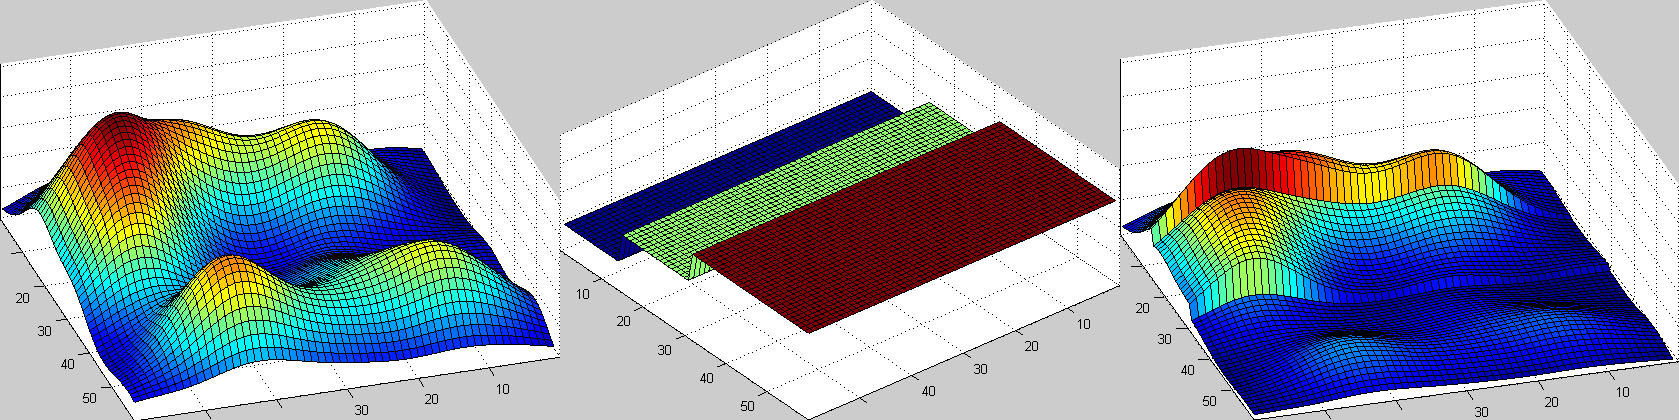
\includegraphics[width=6in]{Multimodal1.jpg}
\caption{A synthetic WiSAR scenario. Left: Multi-modal probability distribution. Middle: A simple task-difficulty map. Right: Probability collectible on first visit (combining probability distribution and task-difficulty map).}
\label{SyntheticCase2}
%\vspace*{-1ex}
\end{figure}

In the LHC-GW-CONV and Top2 algorithms we used the same hierarchical coarse-to-fine search technique to speed up the search for the best UAV path. Here we describe the technique in detail using the Top2 algorithm as an example.

The Top2 algorithm is designed to generate paths that force the UAV to visit the top 2 subregions in the search area. First the Mode Goodness Ratio heuristic is used to identify the top 2 search subregions (represented by centroids). Then, shortest path segments from the start location and the end location (optional) to the nearest centroid are created. The algorithm then identifies a point (vertex) equidistant from the two centroids and launches two path planning tasks to plan path segments from each centroid to that point. By allocating different percentages of the remaining flight time to these two path planning tasks, the Top2 algorithm can effectively search within a new dimension of time allocation. When searching in this new dimension, we used the coarse-to-fine search technique to improve search efficiency.

Figure~\ref{SyntheticCase2} shows an example synthetic WiSAR scenario, and Figure~\ref{CoarseToFine} shows how search efficiency (CDP) changes when different amount of flight time (in time steps) is allocated to the first path segment (the total amount of flight time is static). The curve in Figure~\ref{CoarseToFine} resembles a smooth curve with only one mode, meaning the local maximum would be the global maximum. This property allows us to use a coarse-to-fine search technique so we don't have to search exhaustively through the parameter space.

%Fig.\ref{CTFAlg} shows the pseudo-code for the coarse-to-fine search technique.


\begin{figure}
\centering
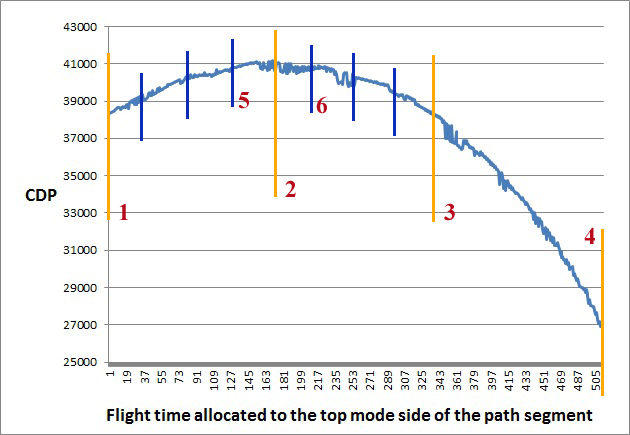
\includegraphics[width=5in]{CoarseToFine.jpg}
\caption{Performance of the Top2 algorithm with the example WiSAR scenario when flight time allocated to first path segment varies.}
\label{CoarseToFine}
%\vspace*{-3ex}
\end{figure}

The coarse-to-fine technique is a recursive method with the number of recursive runs predetermined, depending on what resolution is needed. We start from a low resolution (large chunks of flight time transfered from one path planning task to the other) and gradually increase the resolution (smaller chunks) until the best path is found at the desired resolution. 

First the total flight time is divided into equal chunks (3 chunks in our implementation), then four paths are generated with 0, 1, 2, and 3 chunks of flight time allocated to path segment 1 (remaining time allocated to path segment 2). The performance of these four paths are marked in Figure~\ref{CoarseToFine} relatively by four orange lines labeled 1--4. Then the flight time allocation that generates the best path (maximum CDP) is identified (green line 2). In the next recursive run, the flight time chunk in the previous run is divided into smaller equal chunks, and three more paths are generated at each side of the green line 2 (marked with shorter blue lines). Together with green line 2, performance of these seven paths are compared, and the one with the best path (still green line 2) is identified and will be used as the center for the next recursive round of search (between blue line 5 and 6). With a few recursive runs, the best time allocation point (between blue line 5 and green line 2) can be identified quickly without exhaustively searching through all the possible time allocation options.



%=====================================================================================================
%=====================================================================================================

\chapter{Identifying Modes in a 3D Surface using Local-Hill Climbing with Memory}
\label{chap:modes}


\begin{figure}
\centering
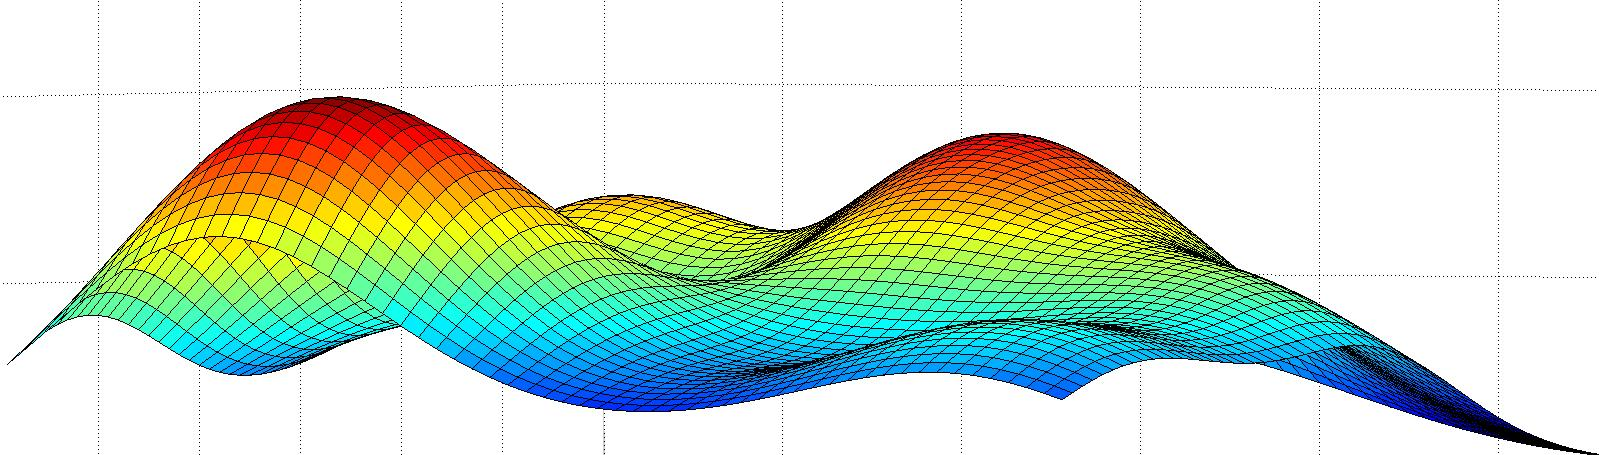
\includegraphics[width=6in]{ExampleSurface.jpg}
\caption{An example 3D surface with 4 modes.}
\label{4modes}
%\vspace*{-1ex}
\end{figure}



A probability density function over a 2D map encodes the probability of certain events in a specific region. For example, the probability density function created for a Wilderness Search and Rescue (WiSAR) operation can show the searchers areas where it is more likely to find the missing person. The distribution map can be used to allocate search resources and to generate flight paths for an Unmanned Aerial Vehicle (UAV). Figure~\ref{4modes} shows an example probability distribution map with 4 modes.

Because different path-planning algorithms may be better suited for different probability distributions~\cite{Wolpert1997No}, identifying the type of distribution beforehand can help us decide what algorithm is appropriate for the specific path-planning task. In our decision process, we particularly care about how many modes the probability distribution has. So how can we automatically identify all the modes in a 3D probability distribution surface? In this appendix we describe the algorithm we use.

In our case, the 3D probability distribution surface is represented by a matrix/table where each value represents the height of the point. You can think of this distribution as a gray-scale image where the gray value of each pixel represent the height of the point.

The \textit{local hill climbing with memory} algorithm proceeds as follows:
\begin{enumerate}
\item \textbf{Downsample and smooth the distribution}: If the distribution map is very large, it is useful to downsample the distribution to improve algorithm speed. For the results in this dissertation, we used $100^2$ sample points over an $100 \times 100$ grid. Since the algorithm assumes that the surface is free of noise, it may be necessary to smooth the surface using a Gaussian filter. The results in this dissertation assume a noise-free surface and, therefore, do not use smoothing.
\item \textbf{Check for a uniform distribution} (a flat surface): It is a good idea to check if the probability distribution is a uniform distribution. Just check to see if all values in the matrix are identical or are within $\varepsilon$ units of each other. If a uniform distribution is identified, we know the distribution has 0 modes and we are done.
\item \textbf{Local Hill Climbing with Memory}: Start from any point of the surface and then check its neighbors (8-connected). As soon as an unvisited neighbor with the same or better value is found, we ``climb'' to that point. As we ``climb'' and check neighbors, we mark all the points we visited along the way. When we check neighbors, we only check points we have not visited before. This way we avoid finding a mode we had found before. The ``climb'' process is repeated until we reach a point (hilltop) where all unvisited neighbors (if there is any) have smaller values. Once we find a ``mode'', we can start from another unvisited point on the surface and do another Local Hill Climbing. Here I use quotes around the word mode because we are not sure if the ``mode'' we found is a real mode, meaning that we have atually found a local maximum of the probability surface.
\item \textbf{Make sure the ``mode'' we found is a real mode}: The ``mode'' we found using Local Hill Climbing might not actually be a real mode. It might be right next to a mode previously found and have a lower value (because we only checked unvisited neighbors in the previous step). It might also be part of another flat-surface mode where the mode consists of multiple points with identical values (think of a hilltop that looks like a plateau or think of a ridge). Things get even more complicated with special distributions such as the example in Figure~\ref{GreatWall}. 

Moreover, the ``mode'' point we found might be connected to a previously found mode through other points with the same value (e.g, the ``mode'' point is the end point of the short branch in the middle of Figure~\ref{GreatWall}). Therefore, we need to keep track of all points leading to the final ``mode'' point that have identical values and check all the visited neighbors of these points, making sure this flat surface is not part of a previously found mode. If these points make up a real new mode, we mark these points with a unique mode count id (e.g, mode 3). If they are only part of a previously found mode, we mark these points with the previously found mode id (e.g., mode 2). If one of them is right next to a previously found mode but has lower value, we mark these points as non-mode points. This step is almost like performing a connected-component labeling operation in Computer Vision~\cite{Sonka2007Image}.
\end{enumerate}

At the end of the algorithm run, we will have a count of how many modes the probability distribution has (maximum mode id) and also a map with all the mode points marked.

\begin{figure}
\centering
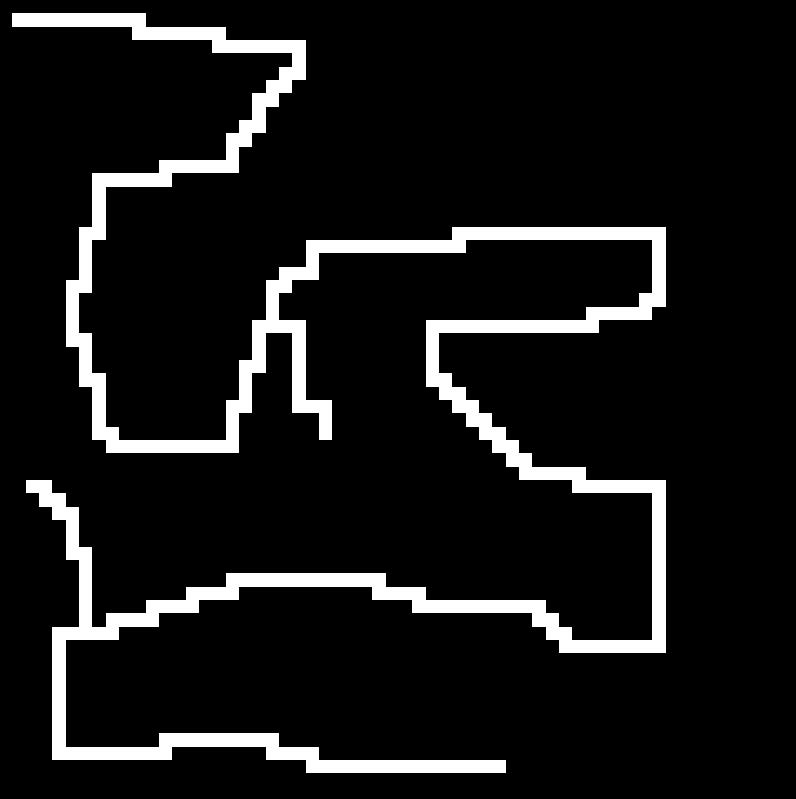
\includegraphics[width=5.5in]{GreatWall.jpg}
\caption{An example path-type distribution resembling the Great Wall of China.}
\label{GreatWall}
%\vspace*{-1ex}
\end{figure}



%=====================================================================================================
%=====================================================================================================

\chapter{Sliding Autonomy User Study Design and Full Results}
\label{chap:SlidingAutonomy}

